\subsection{UC4 - Visualizzazione libreria}
\begin{figure}[H]
  \centering
  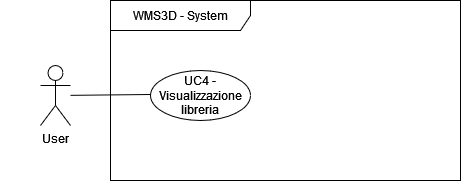
\includegraphics[width=0.8\textwidth]{UC_diagrams_1-10/UC4_sys.drawio.png}
   \caption{Diagramma UML UC4}
\end{figure}
\begin{figure}[H]
  \centering
  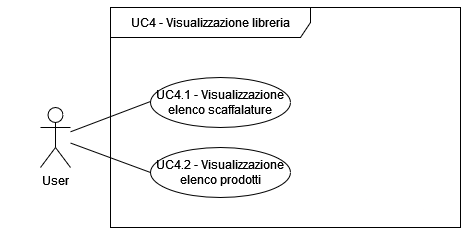
\includegraphics[width=0.8\textwidth]{UC_diagrams_1-10/UC4.drawio.png}
   \caption{Diagramma UML UC4 - dettaglio}
\end{figure}
\begin{itemize}
    \item \textbf{Attori:} User.
    \item \textbf{Pre-condizione:}  L'utente ha creato un magazzino [UC1].
    \item \textbf{Post-condizione:} L'utente visualizza in una parte dell'applicazione uno spazio riservato alle informazioni testuali riguardanti gli elementi (scaffalature e prodotti) interni al magazzino (i.e. la libreria\textsuperscript{G}).
    \item \textbf{Scenario Principale:}  L'utente può visualizzare in libreria\textsuperscript{G}, un elenco delle scaffalature [UC4.1] e uno dei prodotti [UC4.2] (con relativi dati), sempre se presenti all'interno del magazzino. Se non vi dovessero essere nessuno di questi elementi, lo spazio verrà visualizzato vuoto.
    \item \textbf{Generalizzazioni:} -
    \item \textbf{Estensioni:} -
\end{itemize}


\subsubsection{UC4.1 - Visualizzazione elenco scaffalature}
\begin{figure}[H]
  \centering
  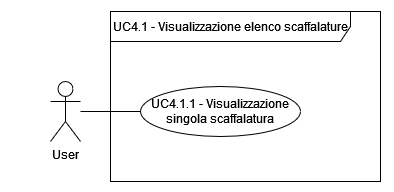
\includegraphics[width=0.8\textwidth]{UC_diagrams_1-10/UC4.1.drawio.png}
   \caption{Diagramma UML UC4.1}
\end{figure}
\begin{itemize}
    \item \textbf{Attori:} User.
    \item \textbf{Pre-condizione:}  L'utente ha creato un magazzino [UC1] e ne sta guardando la libreria.
    \item \textbf{Post-condizione:} L'utente può vedere i dati relativi a tutte le scaffalature presenti nel magazzino.
    \item \textbf{Scenario Principale:} L'utente può visualizzare in libreria\textsuperscript{G} ogni singola scaffalatura [UC4.1.1] (con relativi dati), sempre se presenti all'interno del magazzino. Se non vi dovesse essere nessuna scaffalatura, l'elenco sarà nullo.
    \item \textbf{Generalizzazioni:} -
    \item \textbf{Estensioni:} -
\end{itemize}


\paragraph{UC4.1.1 - Visualizzazione singola scaffalatura}
\begin{figure}[H]
  \centering
  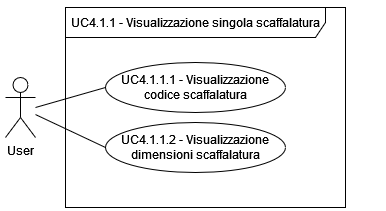
\includegraphics[width=0.7\textwidth]{UC_diagrams_1-10/UC4.1.1.drawio.png}
   \caption{Diagramma UML UC4.1.1}
\end{figure}
\begin{itemize}
    \item \textbf{Attori:} User.
    \item \textbf{Pre-condizione:} L'utente ha creato un magazzino [UC1] e sta guardando all'elenco delle scaffalature interno alla libreria\textsuperscript{G}. Almeno una scaffalatura deve essere creata [UC6] e posizionata [UC7].
    \item \textbf{Post-condizione:} L'utente può vedere i dati relativi ad una singola scaffalatura.
    \item \textbf{Scenario Principale:} L'utente può visualizzare il codice identificativo [UC4.1.1.1] e le dimensioni [UC4.1.1.2] per ogni singola scaffalatura presente nella libreria.
    \item \textbf{Generalizzazioni:} -
    \item \textbf{Estensioni:} -
\end{itemize}


\paragraph{UC4.1.1.1 - Visualizzazione codice scaffalatura}
\begin{itemize}
    \item \textbf{Attori:} User.
    \item \textbf{Pre-condizione:} L'utente ha creato un magazzino [UC1] e sta guardando ad una singola scaffalatura all'interno della libreria\textsuperscript{G}. Pertanto, almeno una scaffalatura deve essere creata [UC6] e posizionata [UC7].
    \item \textbf{Post-condizione:} L'utente può vedere il codice relativo alla singola scaffalatura.
    \item \textbf{Scenario Principale:} L'utente può visualizzare il codice identificativo per ogni singola scaffalatura presente nella libreria.
    \item \textbf{Generalizzazioni:} -
    \item \textbf{Estensioni:} -
\end{itemize}


\paragraph{UC4.1.1.2 - Visualizzazione dimensioni scaffalatura}
\begin{figure}[H]
  \centering
  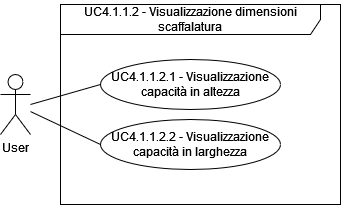
\includegraphics[width=0.8\textwidth]{UC_diagrams_1-10/UC4.1.1.2.drawio.png}
   \caption{Diagramma UML UC4.1.1.2}
\end{figure}
\begin{itemize}
    \item \textbf{Attori:} User.
    \item \textbf{Pre-condizione:} L'utente ha creato un magazzino [UC1] e sta guardando ad una singola scaffalatura all'interno della libreria\textsuperscript{G}. Pertanto, almeno una scaffalatura deve essere creata [UC6] e posizionata [UC7].
    \item \textbf{Post-condizione:} L'utente può vedere le dimensioni relative alla singola scaffalatura.
    \item \textbf{Scenario Principale:} L'utente può visualizzare le dimensioni, quindi capacità in altezza [UC4.1.1.2.1] e capacità in larghezza [UC4.1.1.2.2], per ogni singola scaffalatura presente nella libreria.
    \item \textbf{Generalizzazioni:} -
    \item \textbf{Estensioni:} -
\end{itemize}


\paragraph{UC4.1.1.2.1 - Visualizzazione capacità in altezza}
\begin{itemize}
    \item \textbf{Attori:} User.
    \item \textbf{Pre-condizione:} L'utente ha creato un magazzino [UC1] e sta guardando ad una singola scaffalatura all'interno della libreria\textsuperscript{G}. Pertanto, almeno una scaffalatura deve essere creata [UC6] e posizionata [UC7].
    \item \textbf{Post-condizione:} L'utente può vedere la capacità in altezza relativa alla singola scaffalatura.
    \item \textbf{Scenario Principale:} L'utente può visualizzare la capacità (i.e. numero di bin\textsuperscript{G}) in altezza per ogni singola scaffalatura presente nella libreria.
    \item \textbf{Generalizzazioni:} -
    \item \textbf{Estensioni:} -
\end{itemize}


\paragraph{UC4.1.1.2.2 - Visualizzazione capacità in larghezza}
\begin{itemize}
    \item \textbf{Attori:} User.
    \item \textbf{Pre-condizione:} L'utente ha creato un magazzino [UC1] e sta guardando ad una singola scaffalatura all'interno della libreria\textsuperscript{G}. Pertanto, almeno una scaffalatura deve essere creata [UC6] e posizionata [UC7].
    \item \textbf{Post-condizione:} L'utente può vedere la capacità in larghezza relativa alla singola scaffalatura.
    \item \textbf{Scenario Principale:}  L'utente può visualizzare la capacità (i.e. numero di bin\textsuperscript{G}) in larghezza per ogni singola scaffalatura presente nella libreria.
    \item \textbf{Generalizzazioni:} -
    \item \textbf{Estensioni:} -
\end{itemize}


\subsubsection{UC4.2 - Visualizzazione elenco prodotti}
\begin{figure}[H]
  \centering
  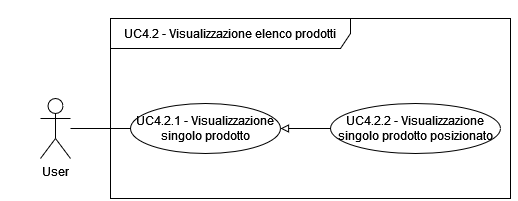
\includegraphics[width=0.8\textwidth]{UC_diagrams_1-10/UC4.2.drawio.png}
   \caption{Diagramma UML UC4.2}
\end{figure}
\begin{itemize}
    \item \textbf{Attori:} User.
    \item \textbf{Pre-condizione:}  L'utente ha creato un magazzino [UC1] e ne sta guardando la libreria.
    \item \textbf{Post-condizione:} L'utente può vedere i dati relativi a tutti i prodotti presenti nel magazzino.
    \item \textbf{Scenario Principale:} L'utente può visualizzare in libreria\textsuperscript{G} ogni singolo prodotto [UC4.2.1] (con relativi dati), posizionato o meno. Se non vi dovesse essere nessun prodotto, l'elenco sarà nullo.
    \item \textbf{Generalizzazioni:} -
    \item \textbf{Estensioni:} -
\end{itemize}


\paragraph{UC4.2.1 - Visualizzazione singolo prodotto}
\begin{figure}[H]
  \centering
  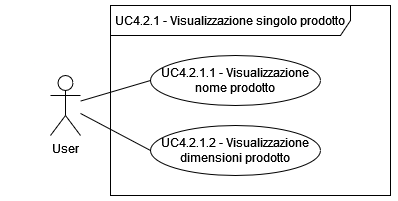
\includegraphics[width=0.8\textwidth]{UC_diagrams_1-10/UC4.2.1.drawio.png}
   \caption{Diagramma UML UC4.2.1}
\end{figure}
\begin{itemize} 
    \item \textbf{Attori:} User.
    \item \textbf{Pre-condizione:}  L'utente ha creato un magazzino [UC1] e sta guardando all'elenco dei prodotti interno alla libreria\textsuperscript{G}. Almeno un prodotto deve essere stato creato [UC13].
    \item \textbf{Post-condizione:} L'utente può vedere i dati relativi ad un singolo prodotto.
    \item \textbf{Scenario Principale:} L'utente può visualizzare il nome [UC4.2.1.1] e le dimensioni [UC4.2.1.2] per ogni singolo prodotto presente nella libreria. 
    \item \textbf{Generalizzazioni:} È presente una generalizzazione:
    \begin{itemize}
        \item UC4.2.2 - Visualizzazione singolo prodotto posizionato
    \end{itemize}
    \item \textbf{Estensioni:} -
\end{itemize}


\paragraph{UC4.2.1.1 - Visualizzazione nome prodotto}
\begin{itemize} 
    \item \textbf{Attori:} User.
    \item \textbf{Pre-condizione:}  L'utente ha creato un magazzino [UC1] e sta guardando ad un singolo prodotto all'interno della libreria\textsuperscript{G}. Almeno un prodotto deve essere stato creato [UC13].
    \item \textbf{Post-condizione:} L'utente può vedere il nome del prodotto.
    \item \textbf{Scenario Principale:} L'utente può visualizzare il nome per ogni singolo prodotto presente nella libreria. 
    \item \textbf{Generalizzazioni:} -
    \item \textbf{Estensioni:} -
\end{itemize}


\paragraph{UC4.2.1.2 - Visualizzazione dimensioni prodotto}
\begin{figure}[H]
  \centering
  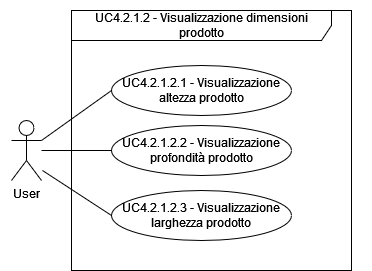
\includegraphics[width=0.8\textwidth]{UC_diagrams_1-10/UC4.2.1.2.drawio.png}
   \caption{Diagramma UML UC4.2.1.2}
\end{figure}
\begin{itemize} 
    \item \textbf{Attori:} User.
    \item \textbf{Pre-condizione:} L'utente ha creato un magazzino [UC1] e sta guardando ad un singolo prodotto all'interno della libreria\textsuperscript{G}. Almeno un prodotto deve essere stato creato [UC13].
    \item \textbf{Post-condizione:}  L'utente può vedere le dimensioni del prodotto.
    \item \textbf{Scenario Principale:} L'utente può visualizzare l'altezza [UC4.2.1.2.1], la profondità [UC4.2.1.2.2] e la larghezza [UC4.2.1.2.3] per ogni singolo prodotto presente nella libreria. 
    \item \textbf{Generalizzazioni:} -
    \item \textbf{Estensioni:} -
\end{itemize}


\paragraph{UC4.2.1.2.1 - Visualizzazione altezza prodotto}
\begin{itemize} 
    \item \textbf{Attori:} User.
    \item \textbf{Pre-condizione:} L'utente ha creato un magazzino [UC1] e sta guardando ad un singolo prodotto all'interno della libreria\textsuperscript{G}. Almeno un prodotto deve essere stato creato [UC13].
    \item \textbf{Post-condizione:}  L'utente può vedere l'altezza del prodotto.
    \item \textbf{Scenario Principale:} L'utente può visualizzare l'altezza per ogni singolo prodotto presente nella libreria. 
    \item \textbf{Generalizzazioni:} -
    \item \textbf{Estensioni:} -
\end{itemize}


\paragraph{UC4.2.1.2.2 - Visualizzazione profondità prodotto}
\begin{itemize} 
    \item \textbf{Attori:} User.
    \item \textbf{Pre-condizione:} L'utente ha creato un magazzino [UC1] e sta guardando ad un singolo prodotto all'interno della libreria\textsuperscript{G}. Almeno un prodotto deve essere stato creato [UC13].
    \item \textbf{Post-condizione:}  L'utente può vedere l'altezza del prodotto.
    \item \textbf{Scenario Principale:} L'utente può visualizzare l'altezza per ogni singolo prodotto presente nella libreria. 
    \item \textbf{Generalizzazioni:} -
    \item \textbf{Estensioni:} -
\end{itemize}


\paragraph{UC4.2.1.2.3 - Visualizzazione larghezza prodotto}
\begin{itemize} 
    \item \textbf{Attori:} User.
    \item \textbf{Pre-condizione:} L'utente ha creato un magazzino [UC1] e sta guardando ad un singolo prodotto all'interno della libreria\textsuperscript{G}. Almeno un prodotto deve essere stato creato [UC13].
    \item \textbf{Post-condizione:}  L'utente può vedere l'altezza del prodotto.
    \item \textbf{Scenario Principale:} L'utente può visualizzare l'altezza per ogni singolo prodotto presente nella libreria. 
    \item \textbf{Generalizzazioni:} -
    \item \textbf{Estensioni:} -
\end{itemize}


\paragraph{UC4.2.2 - Visualizzazione singolo prodotto posizionato}
\begin{figure}[H]
  \centering
  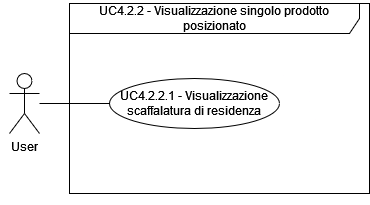
\includegraphics[width=0.8\textwidth]{UC_diagrams_1-10/UC4.2.2.drawio.png}
   \caption{Diagramma UML UC4.2.2}
\end{figure}
\begin{itemize}
    \item \textbf{Attori:} User.
    \item \textbf{Pre-condizione:}  L'utente ha creato un magazzino [UC1] e sta guardando all'elenco dei prodotti interno alla libreria\textsuperscript{G}. Almeno un prodotto deve essere stato creato [UC13] e posizionato [UC14].
    \item \textbf{Post-condizione:}  L'utente può vedere i dati relativi ad un singolo prodotto.
    \item \textbf{Scenario Principale:}  L'utente può visualizzare il nome [UC4.2.1.1] e le dimensioni [UC4.2.1.2] per ogni singolo prodotto ed, essendo posizionato, anche la scaffalatura in cui il prodotto risiede [4.2.2.1]. 
    \item \textbf{Generalizzazioni:} -
    \item \textbf{Estensioni:} -
\end{itemize}


\paragraph{UC4.2.2.1 - Visualizzazione scaffalatura di residenza}
\begin{itemize} 
    \item \textbf{Attori:} User.
    \item \textbf{Pre-condizione:}  L'utente ha creato un magazzino [UC1] e sta guardando ad un singolo prodotto all'interno della libreria\textsuperscript{G}. Almeno un prodotto deve essere stato creato [UC13] e posizionato [UC14].
    \item \textbf{Post-condizione:} L'utente può vedere la scaffalatura di residenza di un prodotto posizionato.
    \item \textbf{Scenario Principale:} L'utente può visualizzare la posizione, ovvero il codice della scaffalatura in cui il prodotto si trova, per ogni singolo prodotto posizionato presente nella libreria. 
    \item \textbf{Generalizzazioni:} -
    \item \textbf{Estensioni:} -
\end{itemize}